\chapter{Solution Overview \\
  \small{\textit{-- Carson McManus}}
  \index{Chapter!solution}
  \index{load balancing}
  \index{load balancer}
  \label{Chapter::SolutionOverview}}

\section{A Smart Load Balancer}

The solution to scaling OTT is to use a load balancer.

\subsection{What is a load balancer?}

A load balancer is a server that distributes load across multiple servers. It is a common solution to the problem of scaling a web application.

\subsection{New Architecture}

With the load balancer, OTT's architecture will look like this: Figure \ref{fig:ott-architecture-with-load-balancer}

\begin{figure}[!h]
  \centering
  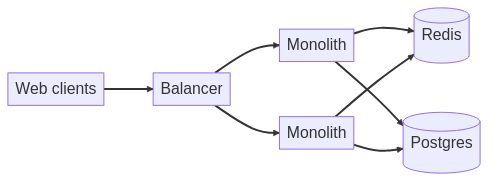
\includegraphics[width=0.4\textwidth]{Figures/ott-architecture-with-load-balancer.png}
  \caption{OTT's architecture with a load balancer}
  \label{fig:ott-architecture-with-load-balancer}
\end{figure}

The load balancer must be able to:
\begin{itemize}
  \item Distribute load across multiple servers
  \item Forward HTTP requests to the correct Monolith
  \item Send WebSocket messages to the correct Monolith
\end{itemize}

These requirements imply that a normal HTTP load balancer (like nginx) will not work, and the need for a specialized implementation. The specifics of how the load balancer will work will be discussed in the following chapters.
